% $Header: /cvsroot/latex-beamer/latex-beamer/examples/beamerexample2.tex,v 1.7 2004/10/07 20:53:07 tantau Exp $

% This file is included by beamerexample2.article.tex and
% beamerexample2.beamer.tex 

% Copyright 2003 by Till Tantau $<$tantau@cs.tu-berlin.de$>$.
%
% This program can be redistributed and/or modified under the terms
% of the LaTeX Project Public License Distributed from CTAN
% archives in directory macros/latex/base/lppl.txt.

%
% The purpose of this example is to demonstrate the usage of the
% nameslide command
%

\mode<article>
{
  \usepackage{fullpage}
  \usepackage{pgf}
  \usepackage{hyperref}
  \usepackage{url}
  \setjobnamebeamerversion{pygtk.beamer}
}

\mode<presentation>
{
  \usepackage{url}
  \usetheme{Madrid}

  \setbeamercovered{transparent}
}

\usepackage[latin1]{inputenc}
\usepackage[spanish]{babel}
\usepackage{fancybox}

\title{Desarrollo de aplicaciones Python-GTK}
\author{Jes�s Espino Garc�a}
\date{12 de Noviembre de 2008}
\subject{Desarrollo de aplicaciones Python-GTK}

\institute[UC3M]{
\includegraphics[height=1.5cm]{gul}}

\begin{document}

  \begin{frame}
    {\maketitle}
  \end{frame}

  \begin{frame}
    \frametitle{Contenidos}

    \begin{itemize}
      \item Introducci�n.
      \item Conceptos b�sicos.
      \item Interfaces.
      \item Algo de c�digo.
      \item Ejemplos.
      \item Referencias.
    \end{itemize}
  \end{frame}

  \begin{frame}
    \frametitle{\begin{center}Introducci�n.\end{center}}
  \end{frame}
  
  \begin{frame}[containsverbatim]
    \frametitle{�Por qu� PyGTK?}

    \begin{itemize}
      \item Es Python!!
      \item Es totalmente libre (Python y GTK).
      \item Es r�pido de aprender.
      \item Es r�pido de desarrollar.
      \item Bien documentado.
      \item Lo aprendido sirve para otros lenguajes.
      \item Es bonito.
      \item Es multi plataforma (Python y GTK)
      \item Si usamos glade, separaci�n de la interfaz del c�digo
    \end{itemize}
  \end{frame}
  
  \begin{frame}
    \frametitle{�Por qu� no?}

    \begin{itemize}
      \item Es Python :(
      \item Ejecuci�n interpretada (lenta)
      \item Proyectos muy grandes (problemas de gran escala)
    \end{itemize}
  \end{frame}
  
  \begin{frame}[containsverbatim]
    \frametitle{�Qu� necesitamos?}
  
    \begin{itemize}
      \item \verb+python+: Interprete de python.
      \item \verb+python-gtk+: Libreria de python GTK.
      \item \verb+glade+: Aplicaci�n de dise�o de interfaces GTK.
      \item \verb+devhelp+: Con el libro de GTK+ una buena referencia.
    \end{itemize}
  \end{frame}

  \begin{frame}
    \frametitle{\begin{center}Conceptos b�sicos.\end{center}}
  \end{frame}
  
  \begin{frame}[containsverbatim]
    \frametitle{Widgets}
  
    Los objetos con los que trabajeremos en GTK
    \begin{itemize}
      \item Ventanas.
      \item Cajas.
      \item Botones.
      \item Entradas.
      \item Etiquetas.
      \item Listas.
      \item Checkboxes.
      \item Otros...
    \end{itemize}
  \end{frame}
  
  \begin{frame}[containsverbatim]
    \frametitle{Contenedores}
  
    Widgets que cotienen otros widgets
    \begin{itemize}
      \item Ventana.
      \item Cajas.
      \item Notebooks.
      \item Otros...
    \end{itemize}
  \end{frame}
  
  \begin{frame}[containsverbatim]
    \frametitle{Se�ales}
  
    Eventos que se producen sobre un widget.
    \begin{itemize}
      \item Clicks.
      \item Pulsado de tecla.
      \item Destruir.
      \item Entrar en el area del widget.
      \item Salir de area del widget.
      \item Moviemiento de raton.
      \item Otros...
    \end{itemize}
  \end{frame}

  \begin{frame}[containsverbatim]
    \frametitle{Manejadores}
  
    Funciones o metodos que gestionan una se�al, es decir, cualquier funci�n o
    metodo definido que se enlaza a la se�al de un objeto.
  \end{frame}

  \begin{frame}
    \frametitle{\begin{center}Interfaces.\end{center}}
  \end{frame}
  
  \begin{frame}[containsverbatim]
    \frametitle{Glade y Gazpacho}

    Interfaz de dise�o de interfaces.
    \begin{itemize}
      \item Es XML.
      \item Es Grafico.
      \item Es GTK.
      \item No pierdes control.
    \end{itemize}

  \end{frame}
  
  \begin{frame}[containsverbatim]
    \frametitle{Glade}
    Interfaz mas popular pues fue el primero en salir en este campo y utiliza
    varias ventanas para realizar su trabajo.
    \begin{center}
      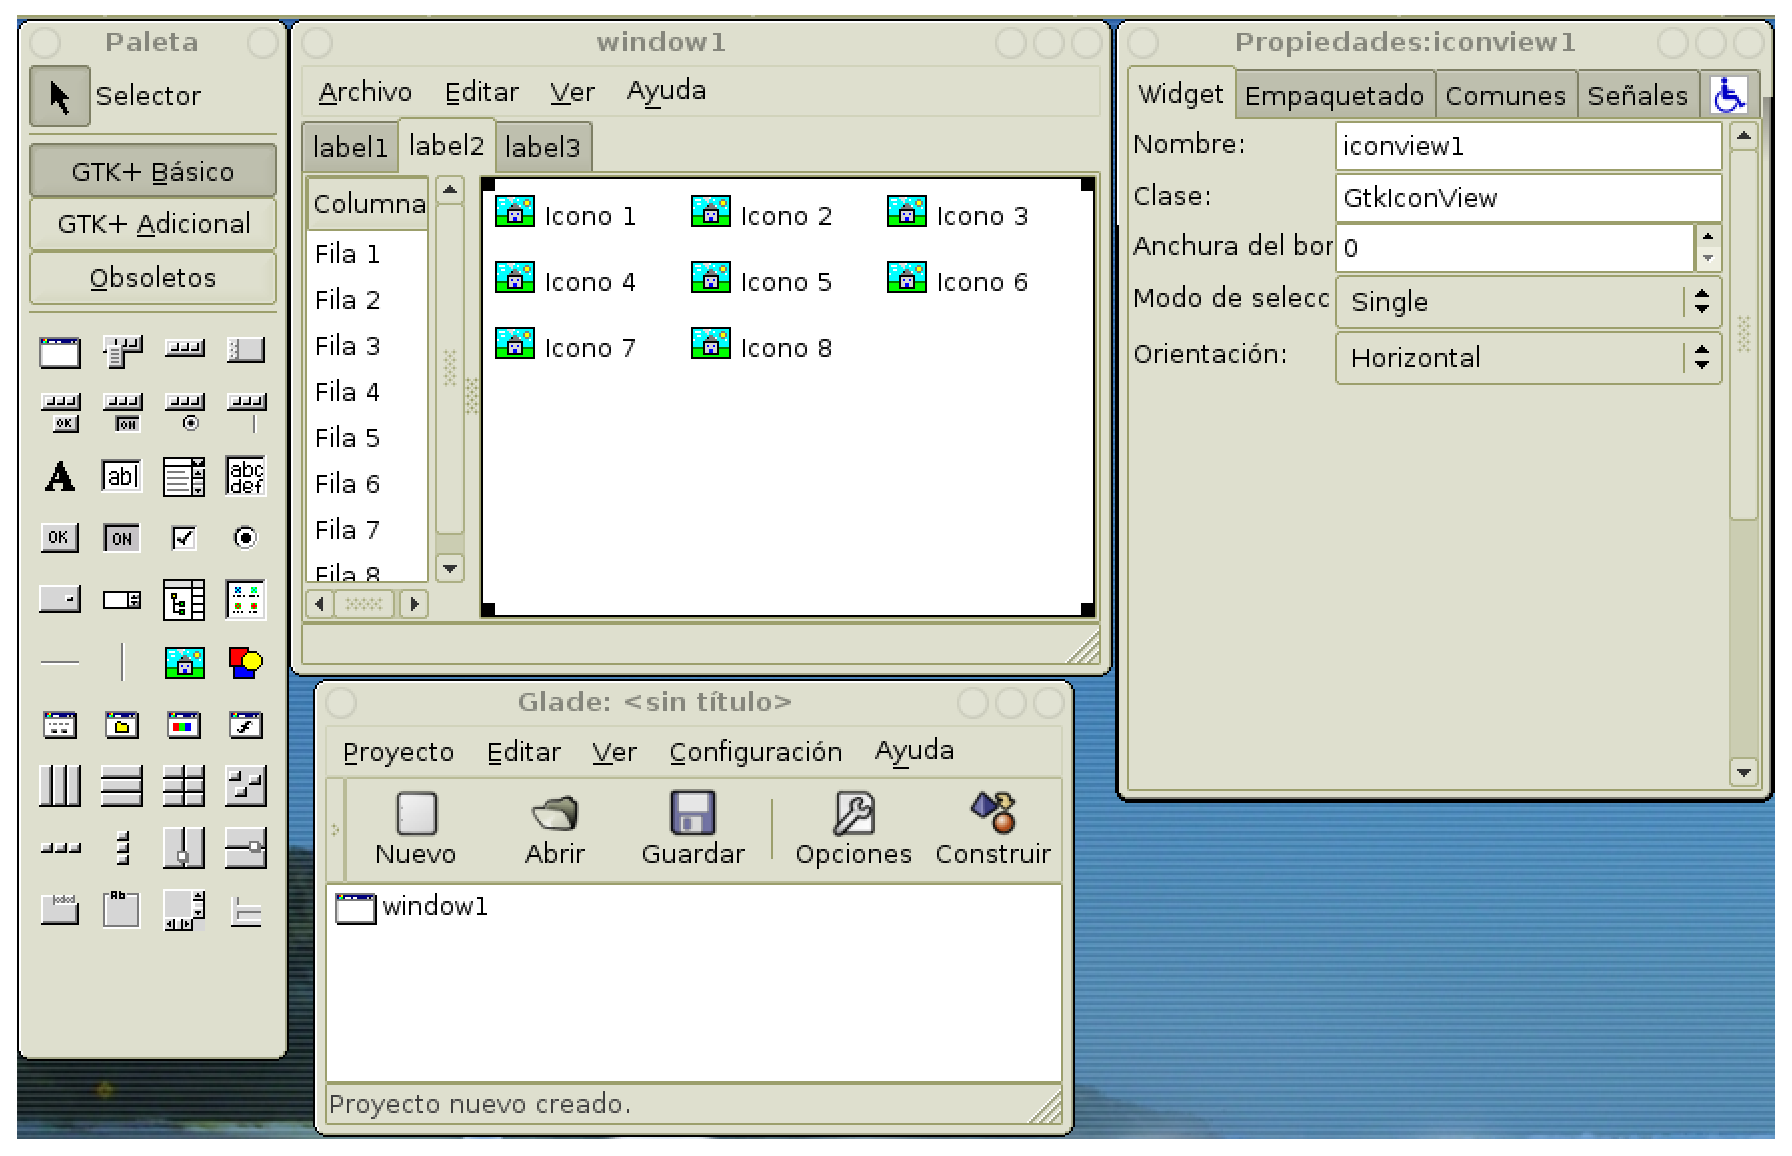
\includegraphics[height=4cm]{glade_shot}
    \end{center}
  \end{frame}
  
  \begin{frame}[containsverbatim]
    \frametitle{Gazpacho}
    Interfaz alternativo, menos utilizado pero una opci�n m�s y utiliza una
    �nica ventanas para realizar su trabajo.
    \begin{center}
      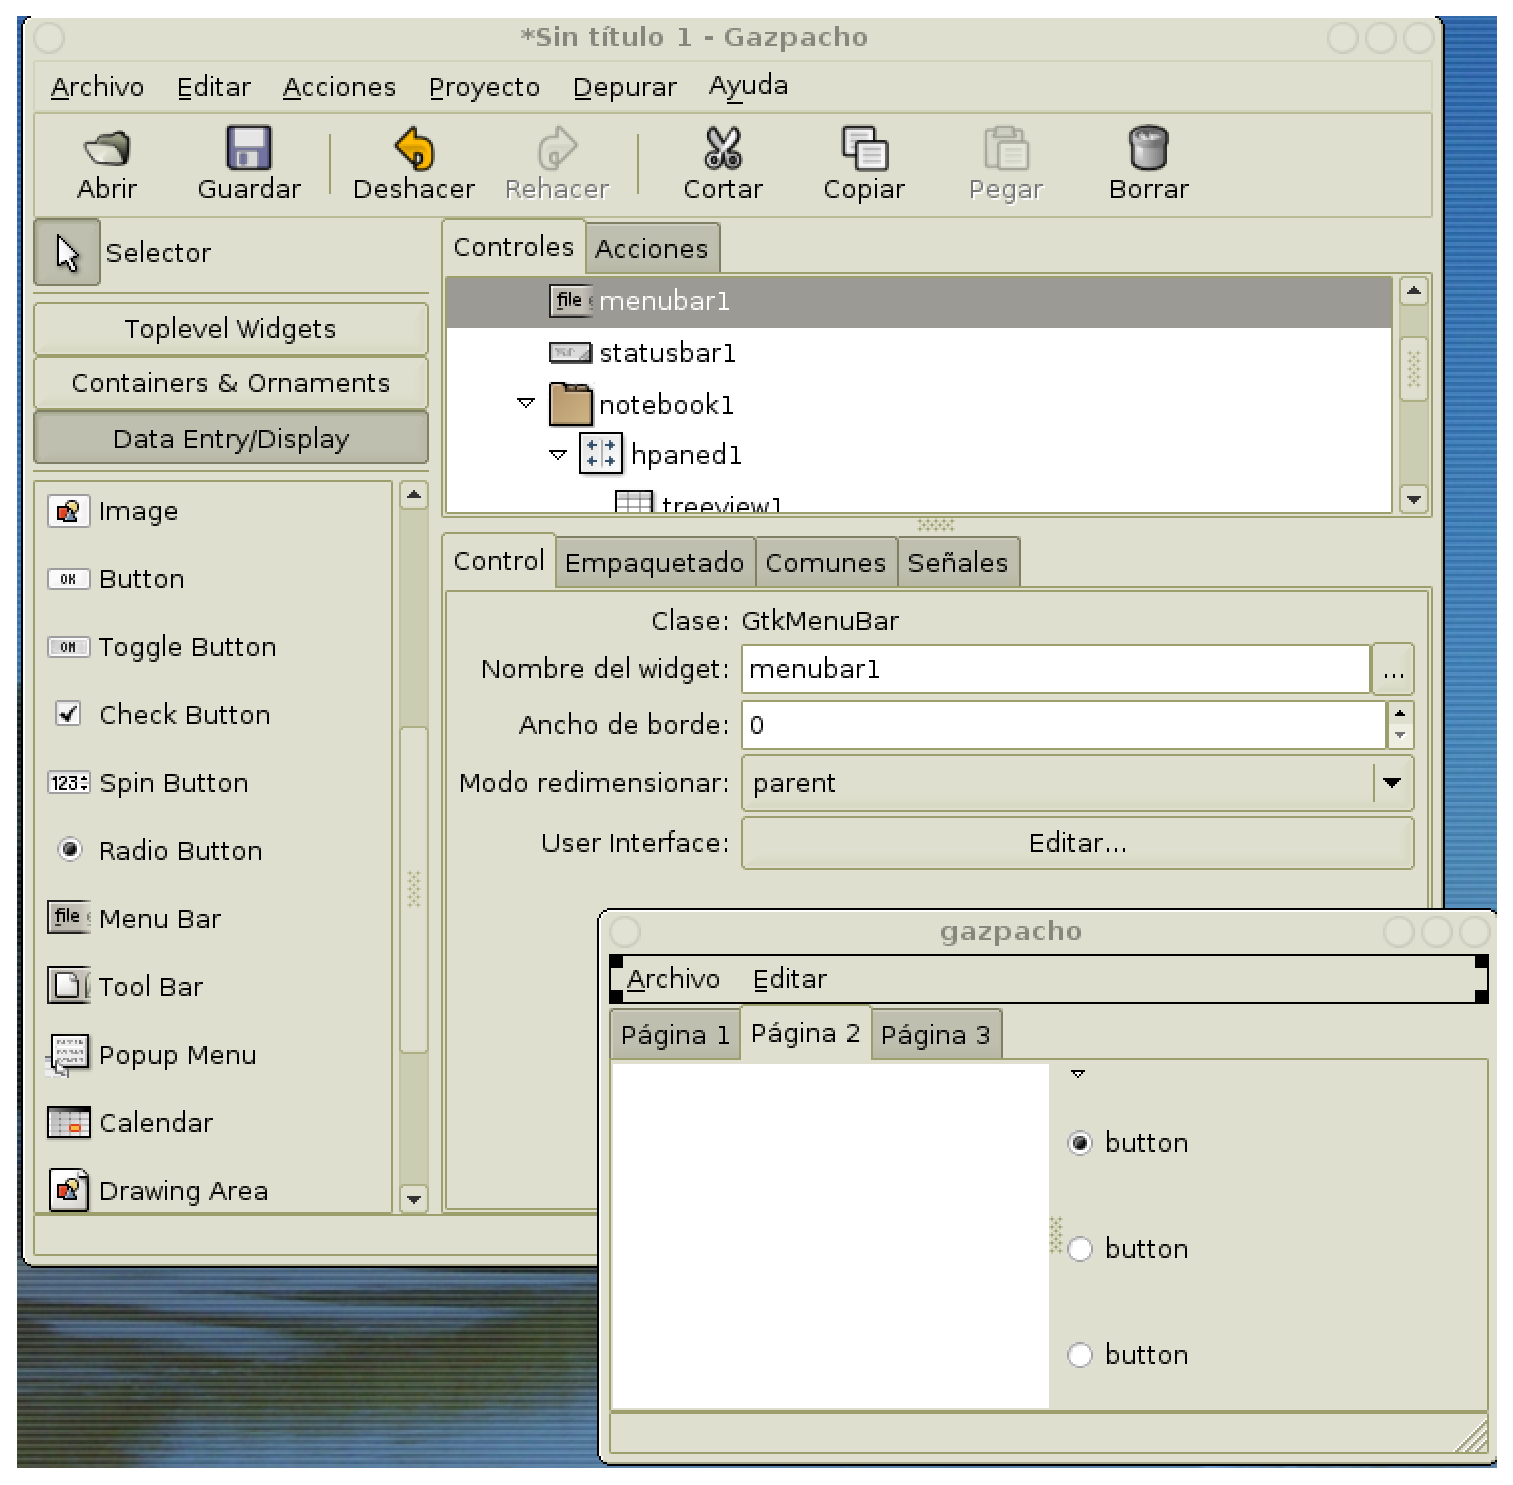
\includegraphics[height=4cm]{gazpacho_shot}
    \end{center}
  \end{frame}
  
  \begin{frame}
    \frametitle{\begin{center}Algo de c�digo.\end{center}}
  \end{frame}
  
  \begin{frame}[containsverbatim]
    \frametitle{B�sico}
    \begin{verbatim}
import gtk

window = gtk.Window()
window.show()

gtk.main()
    \end{verbatim}
  \end{frame}
  
  \begin{frame}[containsverbatim]
    \frametitle{Insertando algun widget}
    \begin{verbatim}
...
button = gtk.Button()
button.show()
window.add(button)
...
    \end{verbatim}
  
  \end{frame}
  
  \begin{frame}[containsverbatim]
    \frametitle{Cambiando informaci�n de un widget.}
    \begin{verbatim}
...
button.set_label("Pulse Aqui")
...
    \end{verbatim}
  \end{frame}
  
  \begin{frame}[containsverbatim]
    \frametitle{Conectando una se�al}
    \begin{verbatim}
...
button.connect("clicked",boton_clickeado)
...
    \end{verbatim}
  \end{frame}

  \begin{frame}[containsverbatim]
    \frametitle{Definiendo un manejador}
    \begin{verbatim}
...
def boton_clickeado(widget):
	print "hola mundo"
...
    \end{verbatim}
  \end{frame}

  \begin{frame}[containsverbatim]
    \frametitle{Importar un interfaz generado}
    \begin{verbatim}
...
xml = gtk.glade.XML("ruta/archivo.glade")
...
    \end{verbatim}
  \end{frame}

  \begin{frame}[containsverbatim]
    \frametitle{Conectar las se�ales}
    \begin{verbatim}
...
xml.signal_autoconnect(locals())
...
    \end{verbatim}
  \end{frame}

  \begin{frame}
    \frametitle{\begin{center}Ejemplos.\end{center}}
  \end{frame}

  \begin{frame}[containsverbatim]
    \frametitle{Mozilla en 30 lineas}
    Ejemplo de insertar un gecko en una aplicaci�n GTK
  \end{frame}

  \begin{frame}[containsverbatim]
    \frametitle{Sumadora}
    Ejemplo de una sumadora que utiliza un XML de glade para generar el interfaz.
  \end{frame}
  
  \begin{frame}
    \frametitle{\begin{center}Para terminar.\end{center}}
  \end{frame}
 
  \begin{frame}
    \frametitle{Referencias}
    \begin{itemize}
      \item �Por d�nde empezar?
        \begin{itemize}
	  \item \url{http://www.pygtk.org}: Referencia completa.
        \end{itemize}
      \item �D�nde preguntar?
        \begin{itemize}
	  \item Lista de correo de pygtk.
	  \item Lista de correo de python.
	  \item Listas de distribuci�n de grupos de usuarios de Linux.
        \end{itemize}
    \end{itemize}
  \end{frame}

  \begin{frame}
    \frametitle{Dudas}
    \dots
  \end{frame}
  
  \begin{frame}
    \frametitle{Agradecimientos}
    \begin{itemize}
      \item Gracias a Pablo Barrera por la charla de Python GTK con la que empec� con esto.
      \item Gracias al equipo de LUC3M por permitirme trabajar en un proyecto tan interesante.
    \end{itemize}
  \end{frame}

  \begin{frame}
    \frametitle{\begin{center}Fin\end{center}}
    \begin{center}
      
\includegraphics[height=3cm]{gul}
    \end{center}
  \end{frame}

\end{document}
